% Drawing 154/02-14 -- folder 154, batch 02, archive page 38 (PDF page 39).
% Transcription: figures : un disque ($D'$, $D$ en haut) accolé par le bas, en un petit segment foncé où $D$ et $D'$ se croisent, à un second disque ($D$, $D'$), puis celui-ci à un troisième ($D'$, $D$ au bas) ; deux disques isolés à droite, reliés par des flèches au crayon aux points de contact
% Kind: chain of three chord systems in disks; two isolated disks. Method 2 (schematic redraw from the facsimile). Status: partial.
% Notes: A disk (D', D at the top) glued at its bottom, in a short dark segment where D and D' cross, to a second disk (D, D'), and this one to a third (D', D at the bottom); two isolated disks on the right joined by pencil arrows to the contact points. Read from the page view; chords and coloured wedges schematic. Still differs from the facsimile: Read from the page view; chords and coloured wedges schematic. 10 coloured or hatched triangle(s) are placed schematically and are not bounded by the strands that bound them on the page.
% Coordinates: 1 unit = 1 mm = 1/100 of the crop width (bbox in page fractions: [0.18, 0.281, 0.356, 0.441]).
% Redrawn by Claude (claude-opus-5-5), issue #73, 2026-11-07; not checked by a human; not compiled (no TeX in the session).
% Revised by Claude (claude-opus-5-5) 2026-11-09 (issue #128) after Michel's check: vertices snapped to exact intersections (drawn points on their lines, meeting ends on the stroke they meet, near-concurrent lines through one computed point, curve ends on their rim); labels at \small as in folder 80 batch 3. Status: partial.
% Rights: reproduces part of the work -- behind RENDER_TRANSCRIPTS, never published by itself.
\documentclass[tikz,border=3pt]{standalone}
\usepackage{amsmath,amssymb}
\usetikzlibrary{patterns,arrows.meta}
\tikzset{Or/.style={orange!90!black}, Ye/.style={yellow!80!orange}, Lg/.style={green!60!black!70}, Dg/.style={green!45!black}, Br/.style={brown!80!black}, Rd/.style={red!85!black}, Bl/.style={blue!70!black}, Gy/.style={black!40}, pencil/.style={black!45}, struck/.style={black!35}, mark/.style={circle,draw,inner sep=1.3pt}, pt/.style={circle,fill,inner sep=0.9pt}, opt/.style={circle,draw,fill=white,inner sep=1.1pt}}
\begin{document}
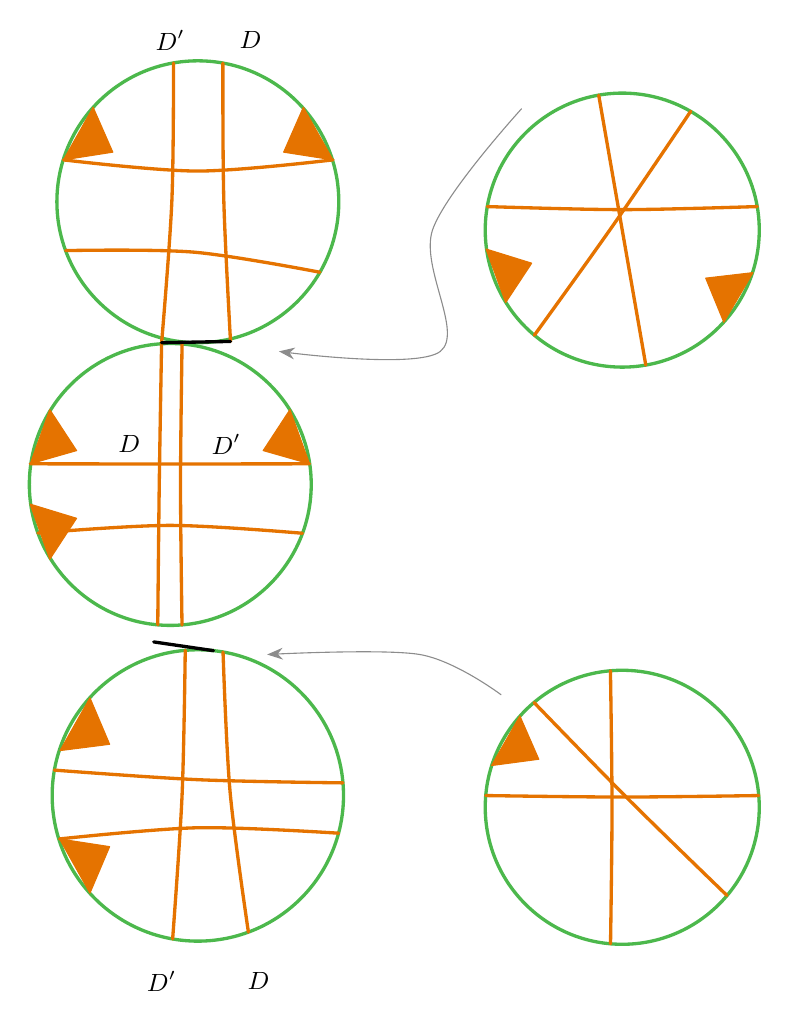
\begin{tikzpicture}[x=1mm,y=1mm,line cap=round,line join=round,font=\scriptsize]
\draw[Lg,very thick] (25.6,-24.6) ellipse[x radius=17.9, y radius=17.9];
\draw[Or,very thick] plot[smooth, tension=0.55] coordinates {(22.51,-6.97) (22.3,-24.5) (21,-42.5)};
\draw[Or,very thick] plot[smooth, tension=0.55] coordinates {(28.78,-6.99) (28.9,-24.5) (29.75,-42.34)};
\draw[Or,very thick] plot[smooth, tension=0.55] coordinates {(8.54,-19.28) (25.6,-20.7) (42.76,-19.28)};
\draw[Or,very thick] plot[smooth, tension=0.55] coordinates {(8.81,-30.8) (25.1,-31) (41.1,-33.55)};
\draw[Or] (12.3,-12.6) -- (8.54,-19.28) -- (14.8,-18.3) -- cycle;
\fill[pattern=north east lines,Or] (12.3,-12.6) -- (8.54,-19.28) -- (14.8,-18.3) -- cycle;
\draw[Or] (42.76,-19.28) -- (39,-12.6) -- (36.5,-18.3) -- cycle;
\fill[pattern=north east lines,Or] (42.76,-19.28) -- (39,-12.6) -- (36.5,-18.3) -- cycle;
\node[inner sep=1pt] at (22.1,-4.1) {\small $D'$};
\node[inner sep=1pt] at (32.3,-4.1) {\small $D$};
\draw[Lg,very thick] (22.1,-60.5) ellipse[x radius=17.9, y radius=17.9];
\draw[Or,very thick] plot[smooth, tension=0.55] coordinates {(21,-42.5) (20.7,-60.5) (20.51,-78.33)};
\draw[Or,very thick] plot[smooth, tension=0.55] coordinates {(23.6,-42.45) (23.4,-60.5) (23.59,-78.34)};
\draw[Or,very thick] plot[smooth, tension=0.55] coordinates {(4.32,-57.88) (22.1,-57.9) (39.78,-57.88)};
\draw[Or,very thick] plot[smooth, tension=0.55] coordinates {(5.3,-66.67) (22.1,-65.7) (38.89,-66.7)};
\draw[Or] (6.8,-51) -- (4.32,-57.88) -- (10.2,-56.2) -- cycle;
\fill[pattern=north east lines,Or] (6.8,-51) -- (4.32,-57.88) -- (10.2,-56.2) -- cycle;
\draw[Or] (39.78,-57.88) -- (37.3,-51) -- (33.9,-56.2) -- cycle;
\fill[pattern=north east lines,Or] (39.78,-57.88) -- (37.3,-51) -- (33.9,-56.2) -- cycle;
\draw[Or] (4.3,-63) -- (6.8,-70) -- (10.2,-64.8) -- cycle;
\fill[pattern=north east lines,Or] (4.3,-63) -- (6.8,-70) -- (10.2,-64.8) -- cycle;
\node[inner sep=1pt] at (16.9,-55.4) {\small $D$};
\node[inner sep=1pt] at (29.2,-55.4) {\small $D'$};
\draw[Lg,very thick] (25.6,-100) ellipse[x radius=18.5, y radius=18.5];
\draw[Or,very thick] plot[smooth, tension=0.55] coordinates {(24,-81.57) (23.6,-99.9) (22.4,-118.22)};
\draw[Or,very thick] plot[smooth, tension=0.55] coordinates {(28.8,-81.78) (29.7,-99.6) (32.02,-117.35)};
\draw[Or,very thick] plot[smooth, tension=0.55] coordinates {(7.38,-96.78) (25.7,-98) (44.03,-98.4)};
\draw[Or,very thick] plot[smooth, tension=0.55] coordinates {(8.04,-105.52) (25.6,-104.1) (43.47,-104.79)};
\draw[Or] (11.9,-87.6) -- (8.1,-94.3) -- (14.4,-93.5) -- cycle;
\fill[pattern=north east lines,Or] (11.9,-87.6) -- (8.1,-94.3) -- (14.4,-93.5) -- cycle;
\draw[Or] (8.04,-105.52) -- (11.9,-112.4) -- (14.4,-106.5) -- cycle;
\fill[pattern=north east lines,Or] (8.04,-105.52) -- (11.9,-112.4) -- (14.4,-106.5) -- cycle;
\node[inner sep=1pt] at (21,-123.6) {\small $D'$};
\node[inner sep=1pt] at (33.3,-123.6) {\small $D$};
\draw[very thick] (21,-42.5) -- (29.75,-42.34);
\draw[very thick] (20,-80.5) -- (27.58,-81.61);
\draw[Lg,very thick] (79.5,-28.2) ellipse[x radius=17.4, y radius=17.4];
\draw[Or,very thick] plot[smooth, tension=0.55] coordinates {(76.51,-11.06) (79.5,-28.2) (82.49,-45.34)};
\draw[Or,very thick] plot[smooth, tension=0.55] coordinates {(62.36,-25.21) (79.5,-25.6) (96.64,-25.21)};
\draw[Or,very thick] plot[smooth, tension=0.55] coordinates {(88.19,-13.12) (78.4,-27.5) (68.34,-41.55)};
\draw[Or] (62.2,-30.6) -- (64.7,-37.4) -- (68,-32.4) -- cycle;
\fill[pattern=north east lines,Or] (62.2,-30.6) -- (64.7,-37.4) -- (68,-32.4) -- cycle;
\draw[Or] (92.4,-39.9) -- (96.1,-33.6) -- (90.1,-34.3) -- cycle;
\fill[pattern=north east lines,Or] (92.4,-39.9) -- (96.1,-33.6) -- (90.1,-34.3) -- cycle;
\draw[Lg,very thick] (79.5,-101.5) ellipse[x radius=17.4, y radius=17.4];
\draw[Or,very thick] plot[smooth, tension=0.55] coordinates {(78,-84.17) (78.2,-101.5) (78.01,-118.84)};
\draw[Or,very thick] plot[smooth, tension=0.55] coordinates {(62.16,-100.01) (79.5,-100.2) (96.84,-100.01)};
\draw[Or,very thick] plot[smooth, tension=0.55] coordinates {(68.29,-88.19) (80.4,-100.6) (92.81,-112.71)};
\draw[Or] (66.5,-89.9) -- (62.9,-96.2) -- (68.9,-95.4) -- cycle;
\fill[pattern=north east lines,Or] (66.5,-89.9) -- (62.9,-96.2) -- (68.9,-95.4) -- cycle;
\draw[pencil,-{Stealth[length=2mm]}] plot[smooth, tension=0.55] coordinates {(66.7,-12.8) (55.4,-28.2) (56.4,-43.6) (35.9,-43.6)};
\draw[pencil,-{Stealth[length=2mm]}] plot[smooth, tension=0.55] coordinates {(64.1,-87.2) (53.8,-82.1) (34.4,-82.1)};
\end{tikzpicture}
\end{document}
